\documentclass[tikz,border=5pt]{standalone}
\usepackage{amsmath}
\usetikzlibrary{arrows.meta,positioning}

\begin{document}
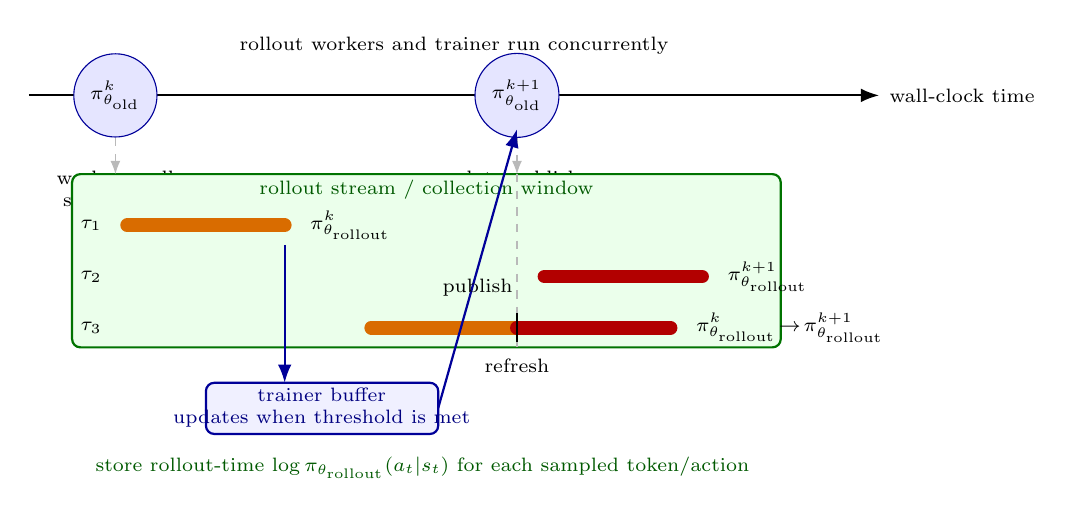
\begin{tikzpicture}[
  font=\scriptsize,
  >=Latex,
  timeaxis/.style={->, thick},
  checkpoint/.style={circle, draw=blue!60!black, fill=blue!10, minimum size=9mm},
  segmenta/.style={line width=5pt, orange!85!black, line cap=round},
  segmentb/.style={line width=5pt, red!70!black, line cap=round},
  guide/.style={dashed, gray!55},
  note/.style={align=center},
  batch/.style={rounded corners=3pt, draw=green!45!black, fill=green!8, thick},
  buffer/.style={rounded corners=3pt, draw=blue!60!black, fill=blue!6, thick}
]

% Wall-clock axis and trainer checkpoints.
\draw[timeaxis] (0,4.45) -- (10.8,4.45) node[right] {wall-clock time};
\node[above] at (5.4,4.85) {rollout workers and trainer run concurrently};

\node[checkpoint] (oldk) at (1.1,4.45) {$\pi_{\theta_{\mathrm{old}}}^{k}$};
\node[checkpoint] (oldkp1) at (6.2,4.45) {$\pi_{\theta_{\mathrm{old}}}^{k+1}$};

\node[below=3mm of oldk, note] {workers pull\\snapshot $k$};
\node[below=3mm of oldkp1, note] {update publishes\\snapshot $k+1$};

% Rollout stream.
\draw[batch] (0.55,1.25) rectangle (9.55,3.45);
\node[green!35!black, note] at (5.05,3.25)
  {rollout stream / collection window};

% Pull arrows from trainer checkpoints into the batch.
\draw[->, guide] (oldk) -- (1.1,3.45);
\draw[->, guide] (oldkp1) -- (6.2,3.45);
\draw[guide] (6.2,3.45) -- (6.2,1.25);

% Staggered trajectory intervals.
\node[anchor=east] at (1.05,2.8) {$\tau_1$};
\draw[segmenta] (1.25,2.8) -- (3.25,2.8);
\node[anchor=west] at (3.45,2.8)
  {$\pi_{\theta_{\mathrm{rollout}}}^{k}$};

\node[anchor=east] at (1.05,2.15) {$\tau_2$};
\draw[segmentb] (6.55,2.15) -- (8.55,2.15);
\node[anchor=west] at (8.75,2.15)
  {$\pi_{\theta_{\mathrm{rollout}}}^{k+1}$};

\node[anchor=east] at (1.05,1.5) {$\tau_3$};
\draw[segmenta] (4.35,1.5) -- (6.2,1.5);
\draw[segmentb] (6.2,1.5) -- (8.15,1.5);
\draw[black, thick] (6.2,1.32) -- (6.2,1.68);
\node[anchor=west] at (8.35,1.5)
  {$\pi_{\theta_{\mathrm{rollout}}}^{k}\!\to\!\pi_{\theta_{\mathrm{rollout}}}^{k+1}$};
\node[below=1mm, note] at (6.2,1.32) {refresh};

% Trainer buffer and update.
\draw[buffer] (2.25,0.15) rectangle (5.2,0.8);
\node[blue!50!black, note] at (3.72,0.48)
  {trainer buffer\\updates when threshold is met};
\draw[->, blue!60!black, thick] (3.25,2.55) -- (3.25,0.8);
\draw[->, blue!60!black, thick] (5.2,0.48) -- node[below, black] {publish} (6.2,4.02);

\node[green!35!black, note] at (5.0,-0.28)
  {store rollout-time $\log \pi_{\theta_{\mathrm{rollout}}}(a_t|s_t)$ for each sampled token/action};

\end{tikzpicture}
\end{document}
